\section{Diskussion}
\label{sec:Diskussion}
Die berechneten Viskositäten von Wasser bei Raumtemperatur entsprechen trotz Unsicherheiten nicht
dem Literaturwert $1.0016 \,\unit[inter-unit-product=\cdot]{\milli\pascal\second}$ (Q\cite{wasserVisk}). Die Abweichung, berechnet mit 
\begin{equation}
  \text{Abweichung}= \frac{\text{Messwert}}{\text{Literaturwert}}\, , 
\end{equation}
 für $\eta_{\text{Hoch}}$ 
beträgt ungefähr $16.8 \,\%$. Die Abweichung für $\eta_{\text{Runter}}$ ist ungefähr $16.2 \,\%$. \\ 
Dies kann unter anderem darauf zurückgeführt werden, 
dass die realistischen Messunsicherheiten wesentlich größer sein werden, als in der Auswertung angenommen. Bei der Messung der Fallzeit müsste zum Beispiel auch die 
Reaktionszeit der messenden Person einbezogen werden. Diese kann zu einem signifikanten Fehler führen. Außerdem haben die beiden Glaskugeln viele Dellen, welche 
zu turbulenteren Strömung führen könnten. Das fehlende Material an den Kugeln führt dazu, dass auch die angegebene Masse nicht mehr stimmen könnte. Diese Masse wurde 
außerdem ohne Fehler angegeben, was die Fehlerfortpflanzung verfälscht. 
\\
Die temperaturabhängige dynamischen Viskositäten stimmen ebenfalls nicht mit den Literaturwerten überein. Die Tendenz des Mediums weniger zäh 
zu sein bei höheren Temperaturen ist allerdings gleich, wie in der untenstehenden Tabelle (\ref{tblr:VergleichViskositaet}) zu sehen. Daher ist es wahrscheinlich, dass der größte Teil der Abweichung dadurch zustande kommt, 
dass das destillierte Wasser zum Zeitpunkt der Messung noch nicht die Temperatur des umliegenden Wassers angenommen hat. Zusätzlich wird die Ungenauigkeit
durch die Reaktionszeit der messenden Person erhöht, wie bei $\eta_{\text{Hoch}}$ und $\eta_{\text{Runter}}$. 
 \\
\begin{table}[H]
    \centering 
    \caption{Vergleich der berechneten dynamischen Viskositäten und der Literaturwerte}
    \begin{tblr}{colspec={c c c c}}
        \toprule
        $T\, \left[\unit{\celsius}\right]$ & $\eta\left(T\right)\, \left[ \unit[inter-unit-product=\cdot]{\milli\pascal\second}\right] $ & $\eta_{\text{lit}}\left(T\right)\, \left[ \unit[inter-unit-product=\cdot]{\milli\pascal\second}\right]$ (Q\cite{wasserVisk})\\
        \midrule
        31\pm1 & 0.962 \pm 0.014 & 0.7805\\
        33\pm1 & 0.908 \pm 0.011 & 0.7488\\
        34\pm1 & 0.907 \pm 0.012 & 0.7337\\  
        36\pm1 & 0.882 \pm 0.011 & 0.7050\\
        40\pm1 & 0.821 \pm 0.010 & 0.6527\\
        42\pm1 & 0.795 \pm 0.010 & 0.6300\\
        43\pm1 & 0.772 \pm 0.009 & 0.6186\\
        44\pm1 & 0.762 \pm 0.010 & 0.6072\\
        47\pm1 & 0.729 \pm 0.011 & 0.5761\\
        49\pm1 & 0.703 \pm 0.009 & 0.5564\\
        \bottomrule
        \label{tblr:VergleichViskositaet}
    \end{tblr}
  \end{table}
\section{Originaldaten}
\label{sec:Originaldaten}
\begin{figure}[H]
  \centering
  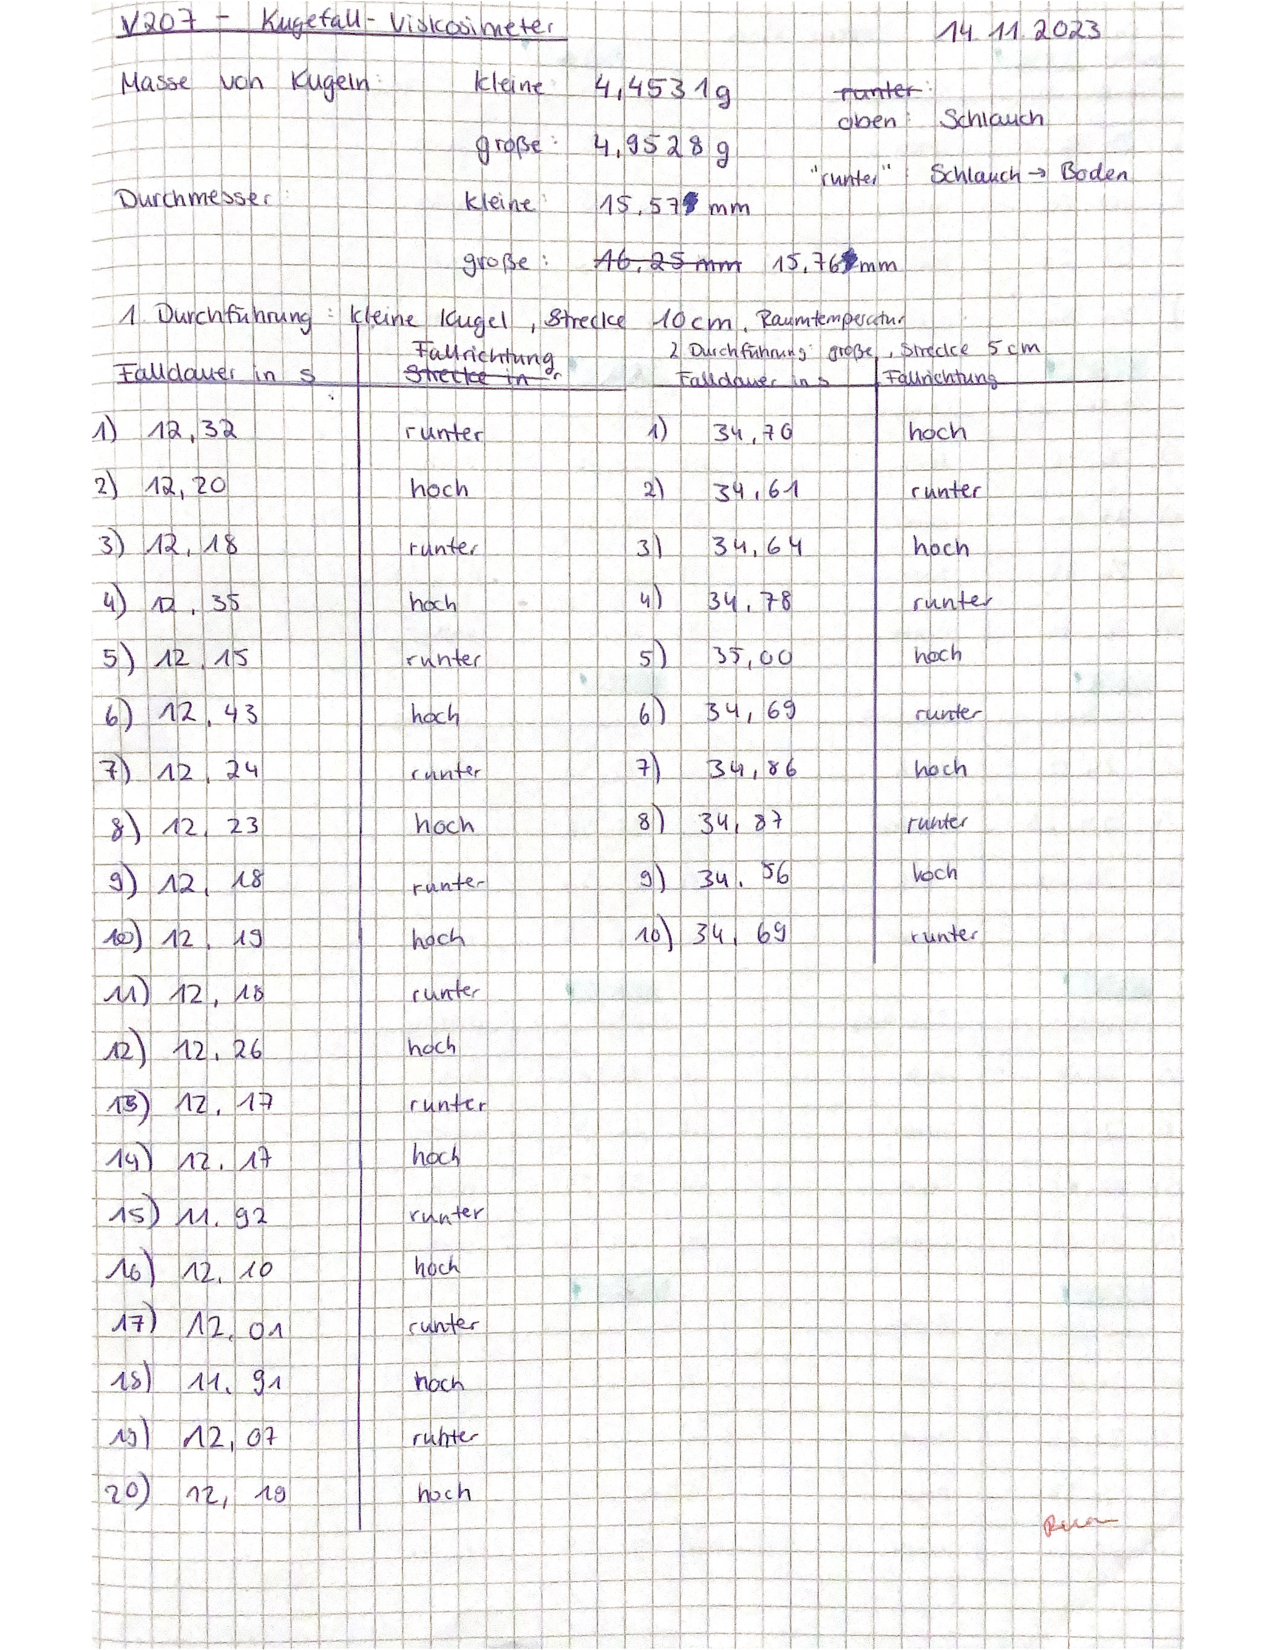
\includegraphics[width=\textwidth]{Messwerte_1.pdf}
  \label{fig:Messungen_1}
\end{figure}
\begin{figure}[H]
  \centering
  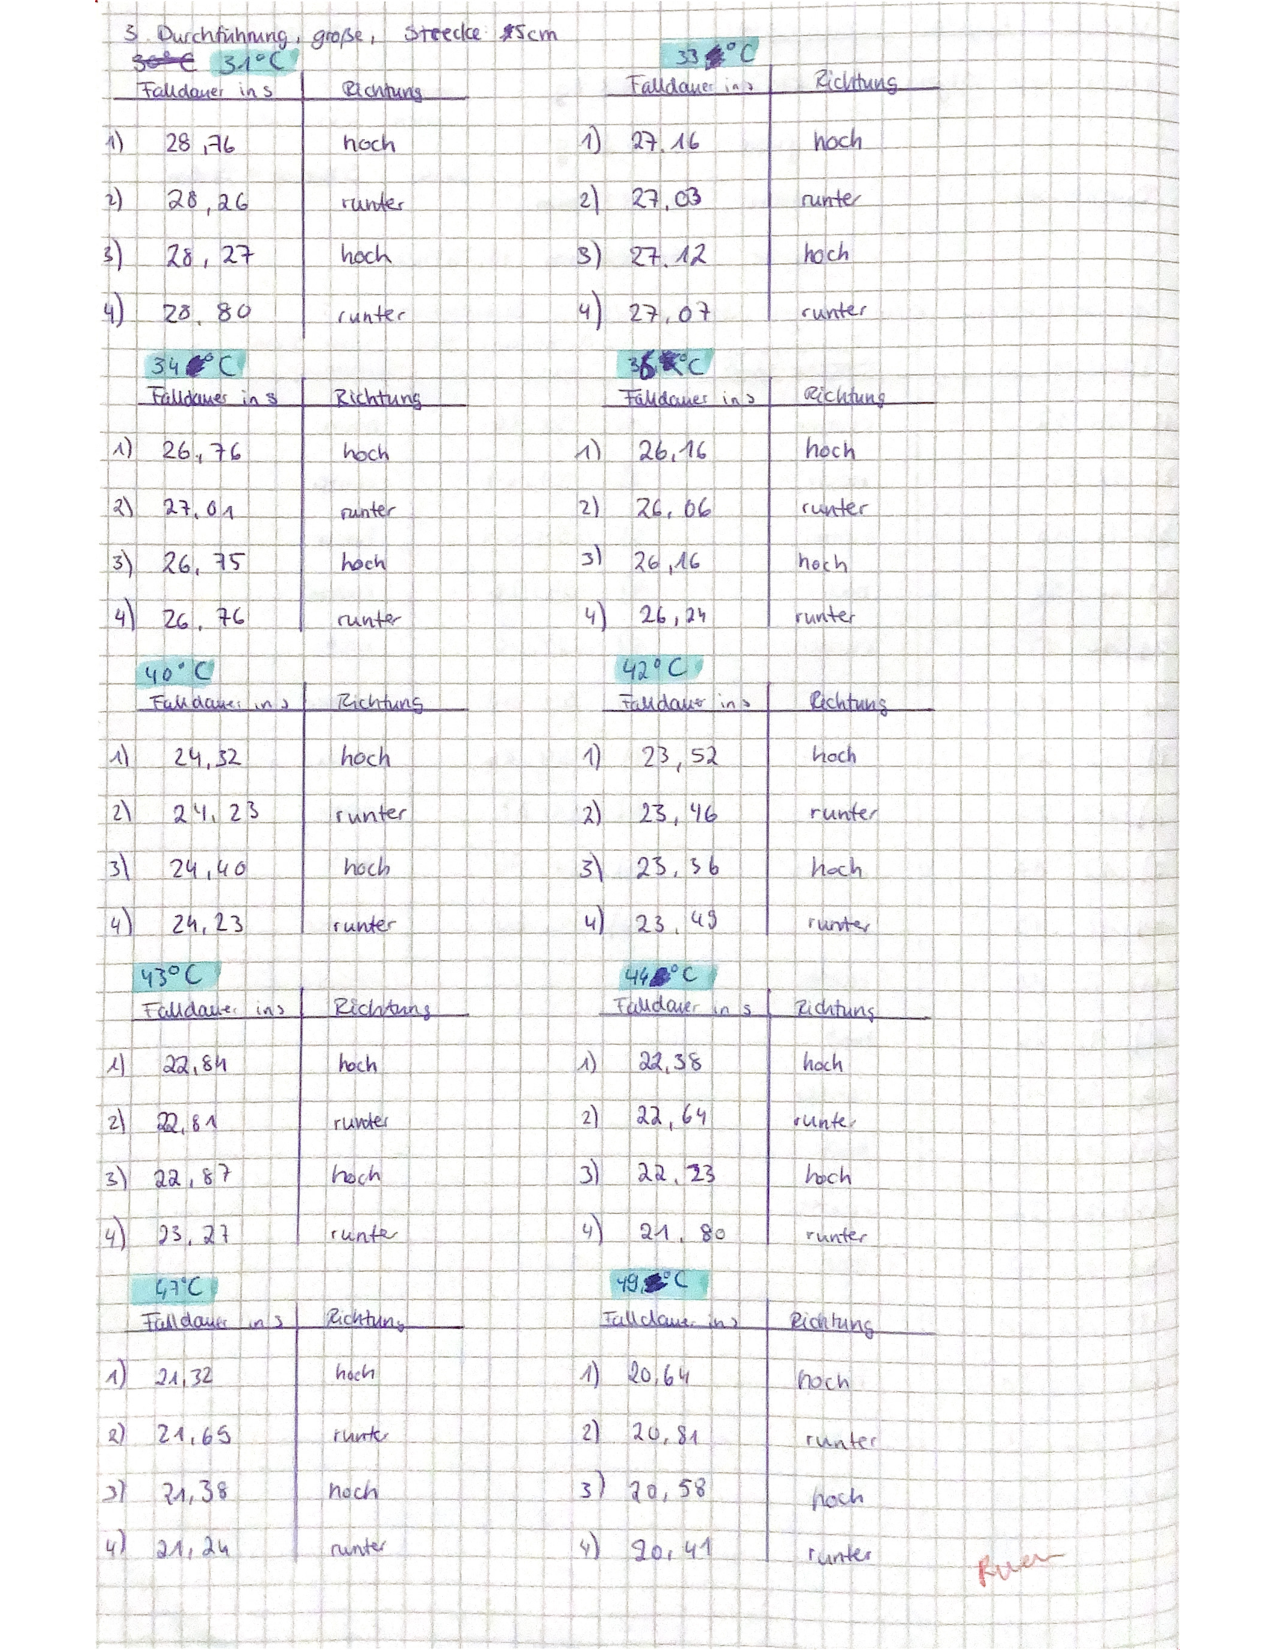
\includegraphics[width=\textwidth]{Messwerte_2.pdf}
  \label{fig:Messungen_2}
\end{figure}